\documentclass{instructions}

\usepackage{alltt}
\usepackage{xspace}

\newcommand{\git}{\texttt{git}\xspace}
\newcommand\bs{\char`\\}

\graphicspath{{figs/}}

\title{Practical 5: Stepper motors and Arduino}
\date{\today}

\summary{
During this lab, you will learn how to control a stepper motor with the Arduino
Uno and the Arduino motor shield.
}

\objectives{
At the end of the lab, you should:

\begin{itemize}
    \item Know how to wire a bipolar or an unipolar stepper motor
    \item Know the different operation modes of a stepper motor and their main
        characteristics
    \item Program a stepper motor controller for the Arduino
\end{itemize}
}

\challenges{

    \begin{itemize}
            \item This lab mostly involve coding; the coding is a bit more
                involved than for the previous labs. A pencil and a piece of
                paper will prove useful.
    \end{itemize}
}

\begin{document}

\maketitle


\note{
    As usual, \textbf{document in your lab journal your findings}.
Add \textbf{code snippets}, \textbf{screenshots}, \textbf{pictures} and link to \textbf{videos} as needed.

\vspace{1em}

And do not forget: \textbf{write your lab journal as a text file using the Markdown
syntax} and \textbf{push your journal and the pictures on GitHub}.

}

%%%%%%%%%%%%%%%%%%%%%%%%%%%%%%%%%%%%%%%%%%%%%%%%%%%%%%%%%%%%%%%%%%
%%%%%%%%%%%%%%%%%%%%%%%%%%%%%%%%%%%%%%%%%%%%%%%%%%%%%%%%%%%%%%%%%%
%%%%%%%%%%%%%%%%%%%%%%%%%%%%%%%%%%%%%%%%%%%%%%%%%%%%%%%%%%%%%%%%%%

\pagebreak

\intro


\step{Sign-out an Arduino + motor shield kit and a stepper motor}

If you have not done so already, sign-out and collect from SMB310 an Arduino Uno
Kit (Arduino Uno, power supply, motor shield) \textbf{and a stepper motor}.

You can keep it for as long as you need to finish all the laboratory sessions.

Return the kit (before the end of term!) when you are done.

\important{\textbf{If you have not finished your DC motor lab}, you still have
until January to complete it: I will not mark the journals before then.
}

\part{Stepper motors: background}

The aim of the lab is to program an Arduino Uno in conjunction with a
motor shield to control a hybrid stepper motor (see Figure~\ref{stepper}).


\begin{figure}[h!]
    \centering
    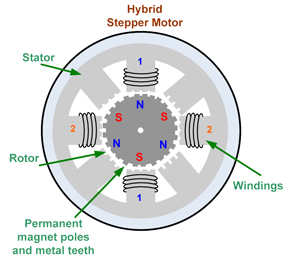
\includegraphics{figs/image3.png}
    \caption{An hybrid stepper motor}
    \label{stepper}
\end{figure}

\begin{itemize}
\item A hybrid stepper motor uses the same control method as a permanent magnet
    stepping motor

\item When a winding is energized, a north and south pole are created

\item The generated poles attract the permanent poles of the rotor on the fine
    metal rotor teeth.

\item The rotor moves one step to align magnetized rotor teeth to the
    corresponding windings.

\item A bipolar motor has four wires. There is no common centre connection and
    it has two independent sets of coils (see Figure~\ref{bipolar}). In this
        case an H-bridge channel on the Arduino motor shield can directly
        control each coil.

\item A unipolar motor has five or six wires. The four coils have a
    common centre connection (see Figure\ref{unipolar}. The common connection(s)
        need to be connected to ground and the other coil connections connected
        to the H-bridge channel on the Arduino motor shield.

\end{itemize}

\begin{figure}[h!]
    \centering
    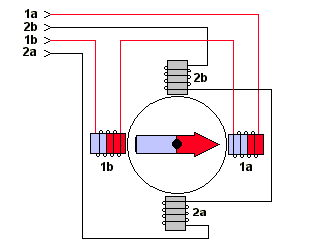
\includegraphics[width=0.5\linewidth]{figs/bipolar.png}
    \caption{A bipolar stepper motor with 4 connection wires}
    \label{bipolar}
\end{figure}


\begin{figure}[h!]
    \centering
    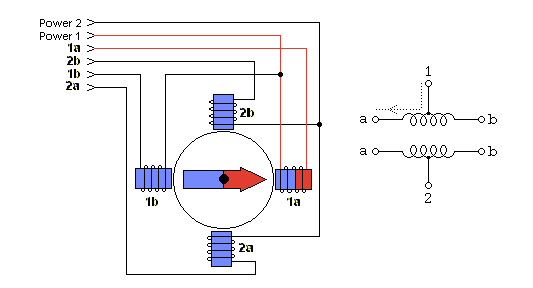
\includegraphics[width=0.7\linewidth]{figs/unipolar.png}
    \caption{A unipolar stepper motor with 5 to 6 connection wires}
    \label{unipolar}
\end{figure}



\part{Control a stepper motor}

\step{Wiring}

Connect the stepper motor to the motor shield (see Figure~\ref{wiring} and
Figure~\ref{connection} for 4-wire bipolar motor). You need to wire it
appropriately depending whether it has a 4 or 6 wires coil connections.

\begin{figure}[h!]
    \centering
    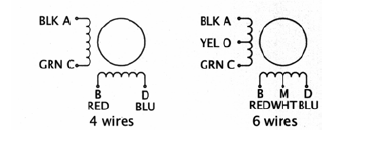
\includegraphics[width=0.7\linewidth]{figs/wiring.png}
    \caption{Wiring diagram for bipolar and unipolar stepper motors}
    \label{wiring}
\end{figure}


\begin{figure}[h!]
    \centering
    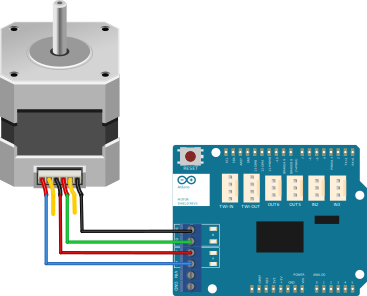
\includegraphics[width=0.7\linewidth]{figs/unipolar-wiring}
    \caption{Connecting the unipolar motor with 6 wires to the motor
  shield. The white and yellow wires are left loose, so that the unipolar motor
    behaves like a bipolar one.}
    \label{connection}
\end{figure}


\step{Initial program}

  Write a program for the Arduino to control its speed and rotational direction.

\step{Programming of modes}

  Write four different functions to implement each of the stepper
  motor control strategies (see diagrams below).

  Implement the following modes:

  \begin{itemize}
  \item Full-step mode (Figure~\ref{fullstep}).
  \item Double-step mode (Figure~\ref{doublestep}).
  \item Half-step mode (Figure~\ref{halfstep}).
  \item Micro-step mode (Figure~\ref{microstep}).
  \end{itemize}

\step{Characterisation}

\begin{itemize}
    \item Estimate the maximum angular velocity of the stepper motor in the different modes

   \item Using your own initiative, roughtly examine the torque of the motor in
        the different modes (Hint: try to stop the shaft rotating by holding
        it with your hand, and compare this across modes).

\end{itemize}


\begin{figure}[h!]
    \centering
    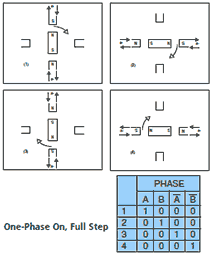
\includegraphics[width=0.4\linewidth]{figs/fullstep.png}
    \caption{Full step mode. Only a single phase is activated at a time.
  As the full step drive, but the motor will have significantly less
    than rated torque}
    \label{fullstep}
\end{figure}


\begin{figure}[h!]
    \centering
    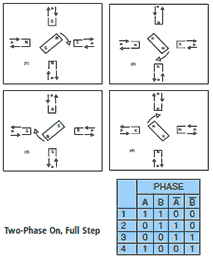
\includegraphics[width=0.4\linewidth]{figs/doublestep.png}
    \caption{Double-step mode. Two phases are always on so the motor will
  provide its maximum rated torque}
    \label{doublestep}
\end{figure}


\begin{figure}[h!]
    \centering
    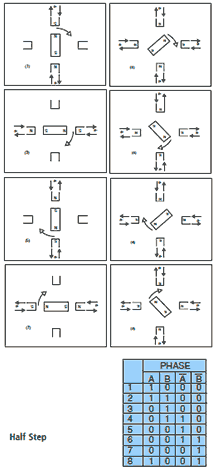
\includegraphics[width=0.4\linewidth]{figs/halfstep.png}
    \caption{Half-step mode. Drive alternates between two phases on and a
single phase on. This increases the angular resolution.}
    \label{halfstep}
\end{figure}


\begin{figure}[h!]
    \centering
    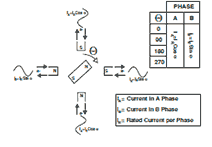
\includegraphics[width=0.4\linewidth]{figs/microstep.png}
    \caption{Microstepping. Winding current approximates a sinusoidal AC
waveform. Motor operation becomes smoother}
    \label{microstep}
\end{figure}



\end{document}
